\chapter{\RU{Указатели}\EN{Pointers}}
\index{\CLanguageElements!\Pointers}
\label{label_pointers}

\RU{Указатели также часто используются для возврата значений из функции (вспомните случай
со \scanf{}~(\myref{label_scanf})).}
\EN{Pointers are often used to return values from functions (recall \scanf case~(\myref{label_scanf})).}
\RU{Например, когда функции нужно вернуть сразу два значения.}
\EN{For example, when a function needs to return two values.}

\section{\RU{Пример с глобальными переменными}\EN{Global variables example}}

\lstinputlisting{patterns/061_pointers/global.c}

\RU{Это компилируется в}\EN{This compiles to}:

\lstinputlisting[caption=\Optimizing MSVC 2010 (/Ob0)]{patterns/061_pointers/global.asm}

\index{\olly}
\clearpage
\RU{Посмотрим это в}\EN{Let's see this in} \olly:

\begin{figure}[H]
\centering
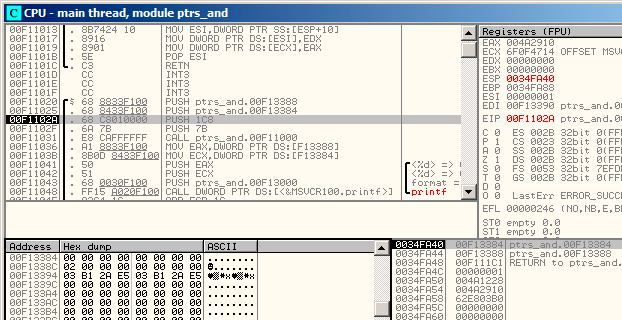
\includegraphics[scale=\FigScale]{patterns/061_pointers/olly_global1.png}
\caption{\olly: \RU{передаются адреса двух глобальных переменных в}
\EN{global variables addresses are passed to} \ttfone}
\label{fig:pointers_olly_global_1}
\end{figure}

\RU{В начале адреса обоих глобальных переменных передаются в}\EN{First, global
variables' addresses are passed to} \ttfone.
\RU{Можно нажать}\EN{We can click} \q{Follow in dump} 
\RU{на элементе стека и в окне слева 
увидим место в сегменте данных, выделенное для двух переменных.}
\EN{on the stack element, and we can see the place in the data segment allocated 
for the two variables.}
\RU{Эти переменные обнулены, потому что по стандарту неинициализированные данные (\ac{BSS}) 
обнуляются перед началом исполнения: \cite[6.7.8p10]{C99TC3}.}

\clearpage
\EN{These variables are zeroed, because non-initialized data (from \ac{BSS}) is cleared before
the execution begins: \cite[6.7.8p10]{C99TC3}.}
\RU{И они находятся в сегменте данных, о чем можно удостовериться, нажав}
\EN{They reside in the data segment, we can verify this by pressing} Alt-M \RU{и увидев карту
памяти}\EN{and reviewing the memory map}:

\begin{figure}[H]
\centering
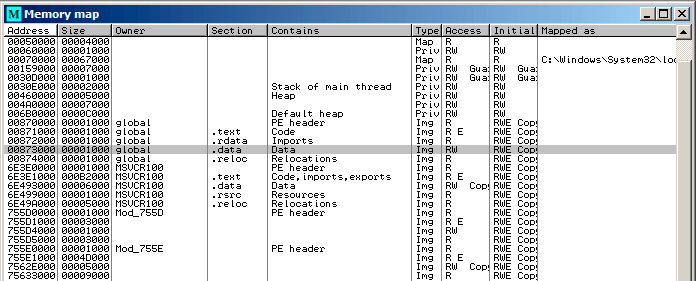
\includegraphics[scale=\FigScale]{patterns/061_pointers/olly_global5.png}
\caption{\olly: \RU{карта памяти}\EN{memory map}}
\label{fig:pointers_olly_global_5}
\end{figure}

\clearpage
\RU{Трассируем}\EN{Let's trace} (F7) \RU{до начала исполнения}\EN{to the start of} \ttfone: 

\begin{figure}[H]
\centering
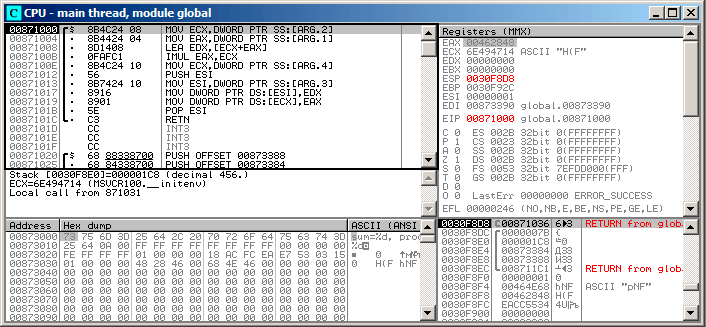
\includegraphics[scale=\FigScale]{patterns/061_pointers/olly_global2.png}
\caption{\olly: \RU{начало работы \ttfone}\EN{\ttfone starts}}
\label{fig:pointers_olly_global_2}
\end{figure}

\RU{В стеке видны значения}\EN{Two values are visible in the stack} 456 (\TT{0x1C8}) \AndENRU 
123 (\TT{0x7B}), \RU{а также адреса двух глобальных переменных}\EN{and also the addresses of the two global variables}.

\clearpage
\RU{Трассируем до конца}\EN{Let's trace until the end of} \ttfone.
\RU{Мы видим в окне слева, как результаты вычисления появились в глобальных переменных}%
\EN{In the left bottom window we see how the results of the calculation appear in the global variables}: 

\begin{figure}[H]
\centering
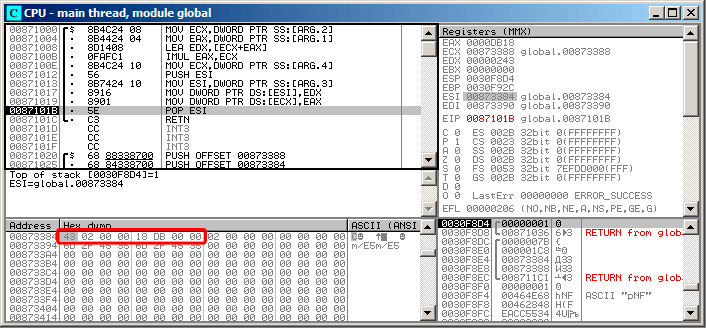
\includegraphics[scale=\FigScale]{patterns/061_pointers/olly_global3.png}
\caption{\olly: \ttfone \RU{заканчивает работу}\EN{execution completed}}
\label{fig:pointers_olly_global_3}
\end{figure}

\clearpage
\RU{Теперь из глобальных переменных значения загружаются в регистры для передачи в}
\EN{Now the global variables' values are loaded into registers ready for passing to} \printf \EN{(via the stack)}:

\begin{figure}[H]
\centering
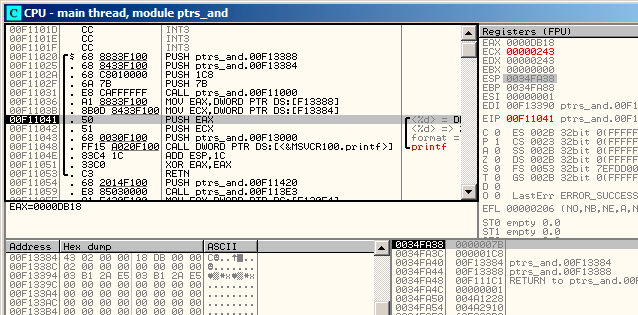
\includegraphics[scale=\FigScale]{patterns/061_pointers/olly_global4.png}
\caption{\olly: \RU{адреса глобальных переменных передаются в}
\EN{global variables' addresses are passed into} \printf}
\label{fig:pointers_olly_global_4}
\end{figure}

\section{\RU{Пример с локальными переменными}\EN{Local variables example}}

\RU{Немного переделаем пример}\EN{Let's rework our example slightly}:

\lstinputlisting[caption=\RU{теперь переменные локальные}
\EN{now the \TT{sum} and \TT{product} variables are local}]{patterns/061_pointers/local.c.\LANG}

\RU{Код функции }\ttfone \RU{не изменится}\EN{code will not change}.
\RU{Изменится только \main}\EN{Only the code of \main will do}:

\lstinputlisting[caption=\Optimizing MSVC 2010 (/Ob0)]{patterns/061_pointers/local.asm}

\newcommand{\PtrsAddresses}{\TT{0x2EF854} \AndENRU \TT{0x2EF858}\xspace}

\clearpage
\RU{Снова посмотрим в}\EN{Let's look again with} \olly.
\RU{Адреса локальных переменных в стеке это}\EN{The addresses of the local variables in the stack are} \PtrsAddresses.
\RU{Видно, как они заталкиваются в стек}\EN{We see how these are pushed into the stack}: 

\begin{figure}[H]
\centering
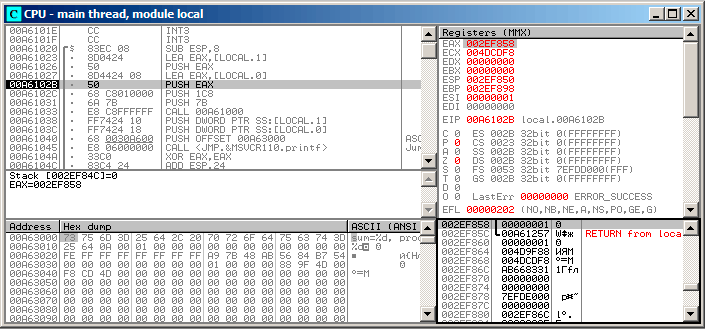
\includegraphics[scale=\FigScale]{patterns/061_pointers/olly_stk1.png}
\caption{\olly: \RU{адреса локальных переменных заталкиваются в стек}\EN{local variables' addresses are
pushed into the stack}}
\label{fig:pointers_olly_stk_1}
\end{figure}

\clearpage
\RU{Начало работы \ttfone}\EN{\ttfone starts}.
\RU{В стеке по адресам}\EN{So far there is only random garbage in the stack at} \PtrsAddresses \RU{пока находится случайный мусор}:

\begin{figure}[H]
\centering
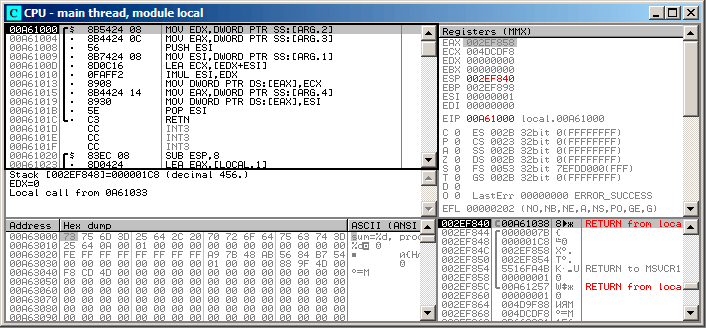
\includegraphics[scale=\FigScale]{patterns/061_pointers/olly_stk2.png}
\caption{\olly: \ttfone \RU{начинает работу}\EN{starting}}
\label{fig:pointers_olly_stk_2}
\end{figure}

\clearpage
\RU{Конец работы \ttfone}\EN{\ttfone completes}:

\begin{figure}[H]
\centering
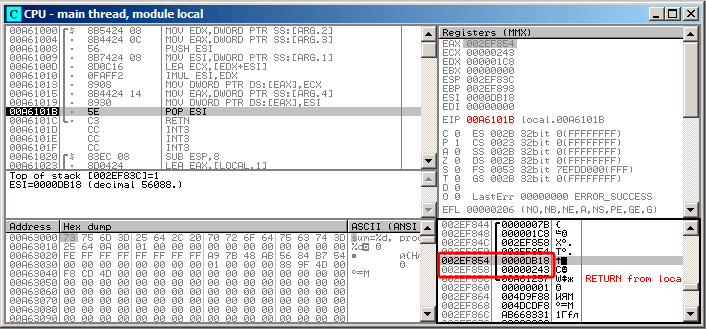
\includegraphics[scale=\FigScale]{patterns/061_pointers/olly_stk3.png}
\caption{\olly: \ttfone \RU{заканчивает работу}\EN{completes execution}}
\label{fig:pointers_olly_stk_3}
\end{figure}

\RU{В стеке по адресам \PtrsAddresses теперь находятся значения \TT{0xDB18} \AndENRU \TT{0x243}, 
это результаты работы \ttfone.}
\EN{We now find \TT{0xDB18} \AndENRU \TT{0x243} at addresses \PtrsAddresses. These values are
the \ttfone results.}

\section{\Conclusion{}}

\RU{\ttfone может одинаково хорошо возвращать результаты работы в любые места памяти.} 
\EN{\ttfone could return pointers to any place in memory, located anywhere.}
\RU{В этом суть и удобство указателей.}
\EN{This is in essence the usefulness of the pointers.}

\RU{Кстати,}\EN{By the way, \Cpp} \IT{references} \RU{в \Cpp работают точно так же}\EN{work exactly the
same way}. \RU{Читайте больше об этом}\EN{Read more about them}: (\myref{cpp_references}).
